% flashcards-title: Distance and displacement on a line
% flashcards-desc: A one-dimensional trip starts at one metre, travels right to five metres, then reverses and ends at negative two metres.
\documentclass[border=7pt]{standalone}
\def\pgfsysdriver{pgfsys-dvisvgm.def}
\usepackage{tikz}
\usetikzlibrary{arrows.meta,positioning,shapes.geometric}
\definecolor{mechInk}{HTML}{172033}
\definecolor{mechBlue}{HTML}{155EEF}
\definecolor{mechOrange}{HTML}{B54708}
\definecolor{mechPale}{HTML}{E8F0FF}
\definecolor{mechGray}{HTML}{667085}
\definecolor{mechLight}{HTML}{D0D5DD}
\tikzset{
  every picture/.style={font=\sffamily\large, text=mechInk},
  mech box/.style={draw=mechInk, line width=1.2pt, rounded corners=4pt,
    fill=white, align=center, minimum height=14mm, inner xsep=5mm},
  mech primary/.style={draw=mechBlue, line width=2.2pt},
  mech secondary/.style={draw=mechOrange, line width=2.2pt, dashed},
  mech guide/.style={draw=mechGray, line width=0.9pt, dashed},
  mech arrow/.style={-{Stealth[length=3.2mm,width=2.4mm]},
    draw=mechInk, line width=1.4pt, line cap=butt},
  mech axis/.style={draw=mechInk, line width=1.2pt},
  mech tick/.style={draw=mechInk, line width=1pt}
}

\begin{document}
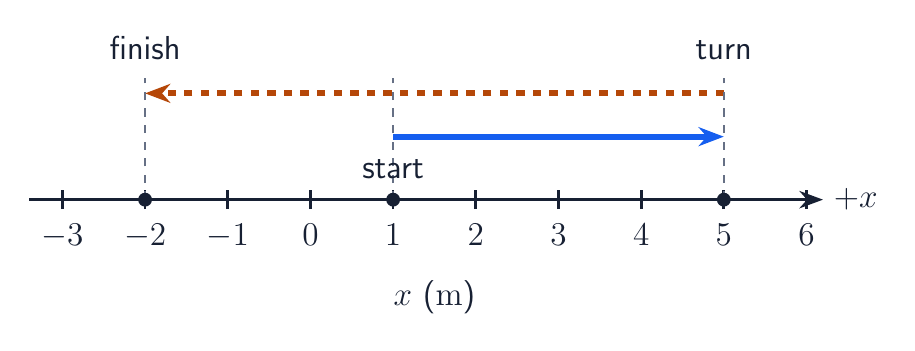
\begin{tikzpicture}[x=1.05cm,y=1cm]
  \draw[mech axis,-{Stealth[length=3mm,width=2.2mm]}] (-3.4,0) -- (6.2,0) node[right] {$+x$};
  \foreach \x in {-3,-2,...,6} {
    \draw[mech tick] (\x,-0.12) -- (\x,0.12);
    \node[below=2pt] at (\x,-0.12) {\(\x\)};
  }
  \node[below=9mm] at (1.5,0) {\(x\) (\(\mathrm{m}\))};
  \draw[mech primary,-{Stealth[length=3.2mm,width=2.4mm]},line cap=butt] (1,0.8) -- (5,0.8);
  \draw[mech secondary,-{Stealth[length=3.2mm,width=2.4mm]},line cap=butt] (5,1.35) -- (-2,1.35);
  \draw[mech guide] (1,0) -- (1,1.55);
  \draw[mech guide] (5,0) -- (5,1.55);
  \draw[mech guide] (-2,0) -- (-2,1.55);
  \fill[mechInk] (1,0) circle (2.5pt);
  \fill[mechInk] (5,0) circle (2.5pt);
  \fill[mechInk] (-2,0) circle (2.5pt);
  \node[above=4pt] at (1,0) {start};
  \node[above=1.65cm] at (5,0) {turn};
  \node[above=1.65cm] at (-2,0) {finish};
\end{tikzpicture}
\end{document}
